The localization and the mapping of the maze are done by a node called Mapper.
It runs at a frequency of $30Hz$ and maps all walls detected by the IR-sensors based on the current pose estimation. The pose is a three dimensional vector $(x,y,\theta)$ describing the robot's position and orientation in a global coordinate system. The pose estimation is mainly based on odometry data. Since this data drifts the Mapper tries to reduce the error by taking the IR data into account.


\subsection{Map}
The maze is built out of linear wall segments and any angle between two non parallel walls is $\frac{\pi}{2}$.
Thus it is possible to separate all walls into two classes: horizontal and vertical walls. Horizontal walls are defined to have an angle of $0$ and vertical walls $\frac{\pi}{2}$. 
The map data structure is based on this constraint and consists out of a list of vertical and horizontal wall segments.

Each wall segment consists out of two points: one start point and one end point. In case of a vertical wall these points have the same $x$-coordinate and in case of a horizontal wall the same $y$-coordinate. Thus the mapped walls have an infinite small thickness. The idea is that the mapped wall segments describe the center of the real walls. For this every distance measurement from an IR sensor is increased by half the wall thickness.  
For convenience it is defined that the start point has the lower $x$($y$)-coordinate and the end point the higher one.

\subsection{Mapping}
The mapping is done while wall following. Since the angles of the walls are strictly defined to be either $0$ or $\frac{\pi}{2}$ the mapping can only be started once the robot is aligned parallel to a wall. As described in section \ref{subsec:wallFollowing} the wall follower has $11$ different states. Every time it changes its state it publishes a message that is received by the Mapper. The first time the wall follower leaves the state \textit{AlignToWall} the Mapper starts mapping. The pose the robot has when this event occurs is defined to be $(0,0,0)$. From there on the pose is first updated based on odometry and then corrected by the Mapper as described in section \ref{subsec:Localization}.

Amee has four short range IR sensors, two on each side. Each sensor is handled separately. Based on the current pose the measured distance is used to calculate the position of where the IR beam is reflected. The approach described in section \ref{subsec:dataAssoc} for data association is then used to associate this measurement with a previously mapped wall. The associated wall is extended so that it contains the new measurement. For horizontal walls the $y$-coordinate and for vertical walls the $x$-coordinate is the average of all the respective measurements' coordinates. 

If no wall fits, a new wall segment is added to the map at this position. The orientation of this new wall segment depends on the current orientation of the robot.

The map stores each type of wall segments in its own list. The list of horizontal walls is ordered by increasing $y$-coordinates and the list of vertical walls by increasing $x$-coordinates. This allows walls that have almost the same $x$(or $y$)-coordinate and overlap or are close to each other to be merged. This compensates drift in the pose estimation and is necessary to merge two wall segments of which one is mapped by the front sensor and the other by the back sensor on one side. 

\subsection{Data association}
\label{subsec:dataAssoc}
The data association is done by ray tracing. Each wall is represented by a line from its start point to its end point. The IR-measurement defines together with the position of the sensor another line, the IR beam. To associate a measurement to a wall it is checked for each wall if the beam and the wall intersect. In case of an incorrect pose estimation the beam might intersect with multiple walls. In that case the measurement is associated to the closest wall to the sensor's position. To allow the wall to grow and to deal with the fact that the mapped wall descibes the real wall's center both the beam and the wall are artificially extended for a couple of $cm$ for this calculation.

\subsection{Localization}
\label{subsec:Localization}
If the data association for both the front and the back sensor on one side is succesful it is possible to correct two components of the pose. The angle relative to the wall can be calculated as $\theta_{rel} = \arctan(\frac{d_{f} - d_{b}}{b})$, where $b$ is the distance between the front and the back sensor, $d_f$ and $d_b$ the measured distances at the front and at the back. Depending on the type and the side of the wall the robot is on, the absolute angle of the wall is either $0$, $\frac{\pi}{2}$,$\pi$ or $\frac{3 \pi}{2}$. With these it is possible to calculate the absolute angle of the robot $\theta$.

If the robot is next to a horizontal wall it is further possible to adapt the robot's $y$-position. In case of a vertical wall it's the $x$-position.
The respective coordinate can be reset based on the measured distance to the wall and the coordinates of this wall. Due to ray tracing it is possible to correct the pose in both cases if it's estimated too close and too far from the wall. 

\subsection{Graph}

For path planning a roadmap defined as directed visibility graph on the map is used. The graph's nodes are placed where one of the following events occurred while mapping: the wall follower aligned to a wall, rotated left or rotated right or a tag was detected. 

The camera node described in section \ref{sect:computerVision} notifies the mapper node about any tag detection. To prevent multiple tag entries into the map at the same position due to multiple detections of the same tag, a tag node is only added if it is at least $0.08m$ away from the last detection. 
The first node added to the graph denotes the entry/exit of the maze.
Each node has an id which uniquely identifies it. The ids are increased every time a new node is added and thus represent the order in which the nodes are added.

Apart from the pose the Mapper provides an additional way of localizing inside of the graph. Every time the wall follower publishes a state change that would result in adding a new node, the distances to all existing nodes of the same type (e.g. rotating right, rotating left, etc..) are checked.
If a previously mapped node of the same type is closer than $0.10m$ and the robot's driving direction is the same, it is assumed that the robot is at the same position as it has been before. This allows to detect whether the robot is moving in a cycle even if the pose estimation drifted a bit. 

Every time a node in the graph is reached a message is published. These messages are later used for path execution as described in \ref{subsubsec:pathExec}.

\subsection{Edges}

By default the nodes of the graph are connected in the order they were added. Thus they represent exactly the path the robot drove while mapping. Once the mapping is done additional edges are added. Two nodes $n_1,n_2$ are connected by an edge $(n_1,n_2)$ if the following requirements are fulfilled:
\begin{itemize}
 \item their distance is less than $0.5m$
 \item $n_1 < n_2$
 \item there is a collision free linear path from $n_1$ to $n_2$.
\end{itemize}

The reasons for the first two constraints are explained in section \ref{pathplanning}. 

The collision checks are executed on the map. For this the line connecting $n_1$ and $n_2$ is sampled. On each sample point the shortest distance to any wall is calculated. This distance is the radius of a collision free circle around the sample point. If it is bigger than the robot's radius plus a small margin, this point can be part of a collision free path, if not it can not and there is no path. This is done for a limited number of sample points until either the complete path is guaranteed to be collision free or a collision was detected.

\begin{figure}
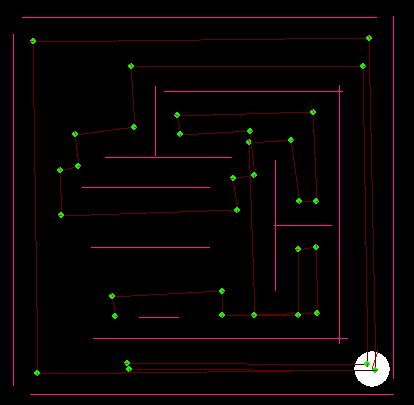
\includegraphics[width=0.5\textwidth]{figures/map_no_edges.png}
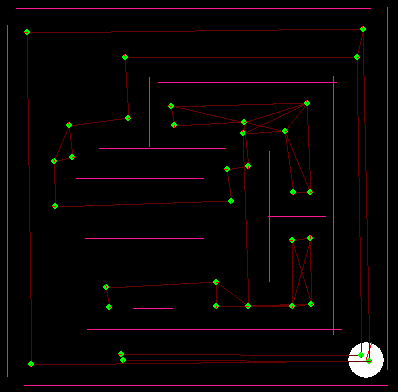
\includegraphics[width=0.5\textwidth]{figures/map_edges.png}
\caption{Map before and after adding of additional edges}
\end{figure}

\subsection{Exploring grid}
The map does only store where walls have been measured, but not where the robot 
has been and where not. It is not guaranteed that the robot will pass all walls inside
of a maze just by wall following. Instead it might occur that there are some areas inside of the
maze that are only reachable by moving freely into unexplored space without following any wall.
To be able to detect such regions an additional data structure called exploration grid is used.
The exploration grid is a binary grid map that stores for cells of a size of
$10cm*10cm$ if they have been explored by the robot or not.
While mapping a cell is set to be explored if one of the following conditions is met:

\begin{itemize}
\item it intersects with the robot
\item it lies between the robot and a cell in which a wall is measured
\item it contains a measured wall on the right side of the robot
\end{itemize}

The cells containing any wall measured on the left side of the robot are not set to be explored. The reason is that the camera is mounted to the right and thus any tag on the left hasn't been detected.


\subsection{Evaluation}

The implemented Mapper node performed in both mapping and localizing very well. The maps of the test mazes turned out to have only few errors, which do not affect the robot’s overall performance. The localization works very well as long as the robot does not move far away from any wall for a longer time period. 

Even if the position drifted, the localization can still recover from it by doing wall following for a time.

The implemented map data structure allows to map mazes with an arbitrary size without requiring any a priori knowledge about it. The representation as set of linear wall segments turned out to be very advantageous as it requires only few memory and allows efficient calculations for the pose correction and collision checking. 

The exploring grid, however, as simple implementation of a grid map adds a lot of disadvantages. It has a predefined maximum number of cells and thus constraints the possible size of mazes the robot can deal with. Although the resolution of the grid is quite low, it needs more memory than the map of the walls. Due to discretization it might also happen that cells are set to be explored although only tiny parts of it were actually explored.

If the robot is next to a wall, it is only possible to correct two out of three components of the pose. While $\theta$ can always be corrected $x$ can only be corrected if the robot is next to a vertical wall and $y$ can only be corrected if it is next to a horizontal wall. Thus if the robot drives parallel to the same wall for a long time, the not corrected component of the pose drifts as it is purely based on odometry.

\begin{figure}
\center
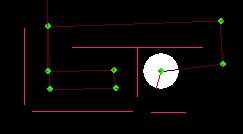
\includegraphics[width=0.5\textwidth]{figures/map_corners.png}
\caption{Map: Gaps in the corners.}
\label{fig:mapGaps}
\end{figure}

As one can see in figure \ref{fig:mapGaps} the mapper does not map corners. This is due to a false data association that occurs while rotating in a corner. When the robot is rotating in a corner for the first time only one of both walls exist in the map. After the robot rotated approximately $45^{\circ}$ the IR measurements that belong to the new not yet mapped wall are still associated to the existing wall. The result would be that the existing wall would be extended to far. The resulting gaps in the map, however, are too small for the robot to fit through. Thus no edges are added to the graph that connect two nodes through such a hole.

For the same reason the localization inside of a corner can only be based on odometry and not on the IR measurements.

\subsection{Possible improvements}

The biggest problem of the localization is the drift of the pose if the robot moves in the same direction for a long time. As explained earlier it is not possible to corrected any pose changes parallel to the followed wall. By using a Kalman filter for the pose estimation this drift could be reduced.

A special modification of the data association while rotating in corners could be introduced to allow corners to be fully mapped.

The exploration grid could be replaced by a quadtree. A good implementation would need less memory and would allow arbitrary maze sizes.



